\documentclass[11pt,a4paper]{article}
\usepackage[utf8]{inputenc}
\usepackage[vietnamese]{babel}
\usepackage{amsmath,amssymb}
\usepackage[version=4]{mhchem}
\usepackage{geometry}
\geometry{top=1.5cm,bottom=1.2cm,left=1.4cm,right=1.4cm,headheight=28pt,headsep=12pt,footskip=18pt}
\usepackage{graphicx}
\usepackage{xcolor}
\usepackage{tabularx}
\usepackage{array}
\usepackage{tikz}
\usepackage{multicol}
\usepackage{fancyhdr}
\usepackage{enumitem}

\definecolor{hfRed}{HTML}{D32F2F}
\definecolor{hfGreen}{HTML}{8BC390}
\definecolor{mainGreen}{HTML}{2E7D32}

\usepackage{ex_test}
\bracketExpl{true}

\pagestyle{fancy}
\fancyhf{}
\renewcommand{\headrulewidth}{0.75pt}
\renewcommand{\headrule}{\hbox to\headwidth{\color{hfGreen}\leaders\hrule height \headrulewidth\hfill}}
\renewcommand{\footrulewidth}{0.75pt}
\renewcommand{\footrule}{\hbox to\headwidth{\color{hfGreen}\leaders\hrule height \footrulewidth\hfill}}

\fancyhead[L]{\small\itshape\color{hfRed}Tài liệu lưu hành nội bộ}
\fancyhead[R]{\small\color{hfRed}Thầy \textbf{TRẦN VĂN THẠNH} - 0777.470.803}

\fancyfoot[L]{\footnotesize\itshape\color{hfRed}CS1: 6/15 Nguyễn Hoàng, P. Kim Long, TP Huế \quad|\quad CS2: 24 Đặng Thái Thân, TP Huế}
\fancyfoot[R]{\small\textbf{\color{hfRed}Trang \thepage}}

\setlength{\parindent}{0pt}
\setlength{\parskip}{2pt}

\def\loigiai#1{}

\begin{document}

\Opensolutionfile{ans}[ans-de07-hs]

\noindent
\begin{minipage}[t]{0.48\textwidth}
	\centering
	\textbf{SỞ GIÁO DỤC VÀ ĐÀO TẠO THỪA THIÊN HUẾ}\\
	\textbf{ĐỀ CHÍNH THỨC}\\
	\textit{(Đề thi có 04 trang)}
\end{minipage}\hfill
\begin{minipage}[t]{0.48\textwidth}
	\centering
	\textbf{\color{mainGreen}ĐỀ KIỂM TRA ĐỊNH KỲ CHƯƠNG 3 (HỢP CHẤT NITROGEN)}\\
	\textbf{MÔN: HOÁ HỌC -- LỚP 12}\\
	\textit{Thời gian làm bài: 50 phút (không kể thời gian phát đề)}\\
	\textbf{Mã đề thi: 107}
\end{minipage}


\vspace{0.1cm}
\noindent\textit{Họ, tên thí sinh: \dots\dots\dots\dots\dots\dots\dots\dots\dots\dots\dots\dots\dots\dots\dots\dots\dots\dots\dots\dots\dots\dots Lớp: \dots\dots\dots\dots SBD: \dots\dots\dots\dots}\\
\noindent\textit{(Cho biết nguyên tử khối: H = 1; C = 12; N = 14; O = 16; Na = 23; S = 32; Cl = 35,5; Fe = 56; Cu = 64).}

\vspace{0.15cm}
\noindent
\textbf{PHẦN I (4,5 điểm -- 18 câu): Câu trắc nghiệm nhiều phương án lựa chọn.}\\
\textit{Thí sinh trả lời từ câu 1 đến câu 18. Mỗi câu hỏi thí sinh chỉ chọn một phương án.}

\setcounter{ex}{0}

\begin{ex}
Chất nào sau đây là amine thơm?
\choice
{Aniline}
{Cyclohexylamine}
{Alanine}
{Trimethylamine}
\loigiai{}
\end{ex}

\begin{ex}
Aniline có công thức phân tử là:
\choice
{\ce{C3H7O2N}}
{\ce{C2H5O2N}}
{\ce{C7H9N}}
{\ce{C6H7N}}
\loigiai{}
\end{ex}

\begin{ex}
Phân tử amine có cấu tạo tương tự phân tử nào sau đây nhất?
\choice
{\ce{H2O}}
{\ce{NH3}}
{\ce{HF}}
{\ce{N2}}
\loigiai{}
\end{ex}

\begin{ex}
Số nhóm amino (-\ce{NH2}) có trong một phân tử Lysine là
\choice
{1}
{3}
{4}
{2}
\loigiai{}
\end{ex}

\begin{ex}
(SBT -- CTST). Ở điều kiện thường, trạng thái tồn tại của amino acid là
\choice
{thể lỏng}
{thể khí}
{thể rắn}
{thể rắn và lỏng}
\loigiai{}
\end{ex}

\begin{ex}
Khi đun nóng, các $\varepsilon$-amino acid hoặc $\omega$-amino acid có thể phản ứng với nhau để tạo thành polymer, đồng thời tách ra các phân tử nước gọi là phản ứng
\choice
{ester hóa}
{trùng ngưng}
{trùng hợp}
{hydrogen hóa}
\loigiai{}
\end{ex}

\begin{ex}
Peptide: \ce{H2NCH2CONHCH(CH3)CONHCH2COOH} được biểu diễn dạng kí hiệu như sau
\choice
{Gly -- Gly -- Ala}
{Gly -- Ala -- Gly}
{Ala -- Gly -- Gly}
{Ala -- Gly -- Ala}
\loigiai{}
\end{ex}

\begin{ex}
Trong phân tử tetrapeptide Gly-Val-Glu-Ala, amino acid đầu C là
\choice
{Gly}
{Val}
{Glu}
{Ala}
\loigiai{}
\end{ex}

\begin{ex}
Insulin, một loại hormone thuộc loại protein, được sản sinh bởi tuyến tuỵ, có chức năng điều hoà quá trình chuyển hoá glucose trong cơ thể. Insulin thúc đẩy sự hấp thu glucose của các tế bào và dự trữ glucose dư thừa trong gan và cơ. Insulin là
\choice
{protein đơn giản}
{protein phức tạp}
{dipeptide}
{monomer}
\loigiai{}
\end{ex}

\begin{ex}
(SBT -- KNTT). Trong cơ thể, enzyme có chức năng nào sau đây?
\choice
{Cấu trúc tế bào}
{Chất điện giải}
{Chất dự trữ năng lượng}
{Xúc tác sinh học}
\loigiai{}
\end{ex}

\newpage

\begin{ex}
(SBT -- CTST). Amine nào sau đây phản ứng được với nitrous acid tạo thành muối diazonium bền ở nhiệt độ thấp?
\choice
{Methanamine}
{Methanediamine}
{Benzenamine}
{Phenylmethanamine}
\loigiai{}
\end{ex}

\begin{ex}
(SBT -- CTST). Dạng ion chủ yếu nào của amino acid có trong môi trường acid mạnh (pH thấp)?
{\centering
	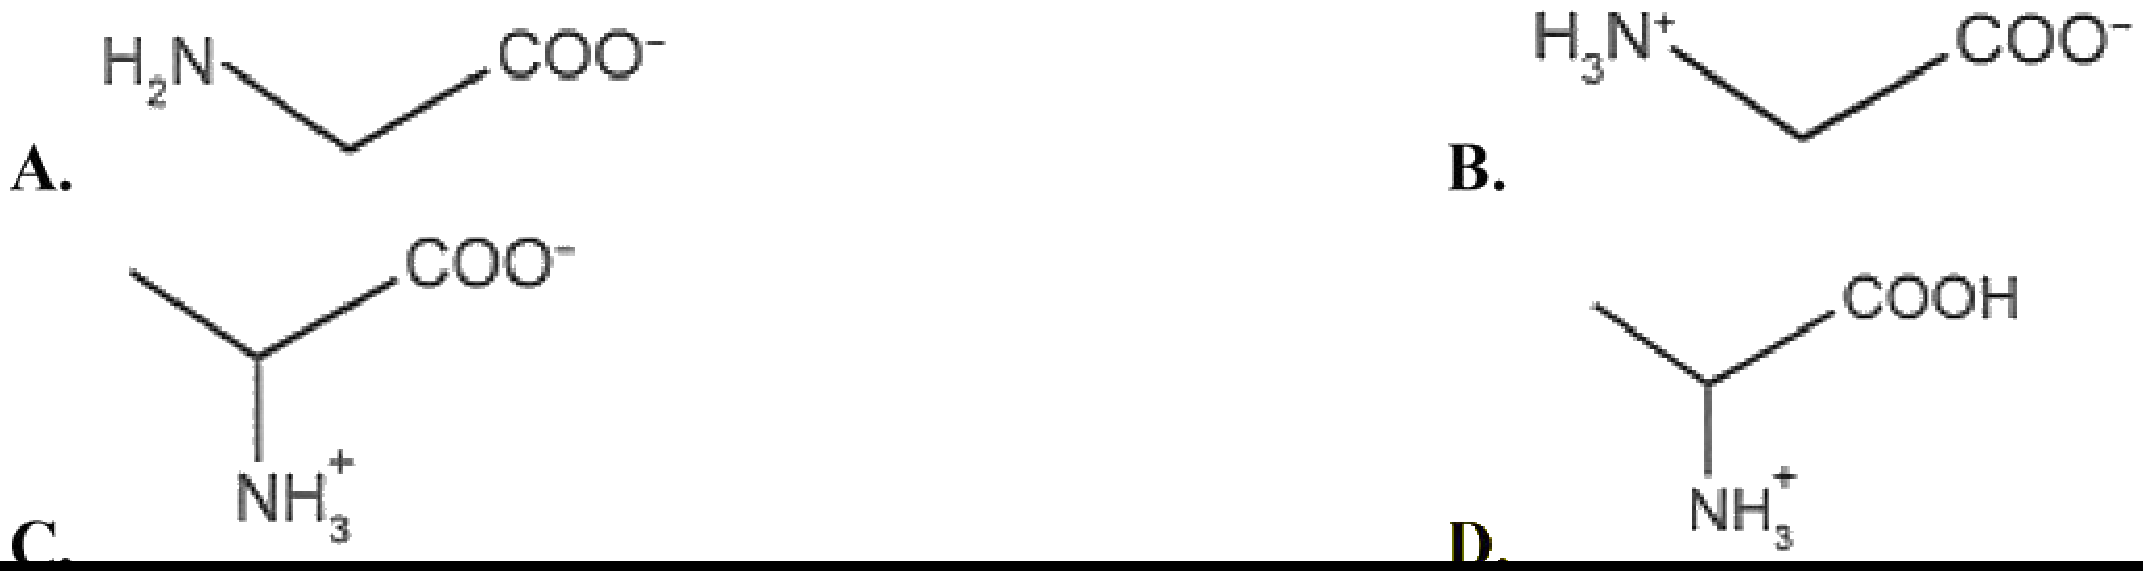
\includegraphics[width=10.0cm]{images_crop_de07/cau12_options.png}\par}
\loigiai{}
\end{ex}

\begin{ex}
(SBT -- CĐ). Một tripeptide X được cấu thành từ 2 phân tử Ala và 1 phân tử Gly. Công thức cấu tạo của X \textbf{không} thể là
\choice
{Ala-Ala-Gly}
{Ala-Gly-Ala}
{Gly-Ala-Ala}
{Gly-Ala-Gly}
\loigiai{}
\end{ex}

\begin{ex}
(SBT -- CĐ). Cho peptide X có công thức cấu tạo như hình bên dưới:
{\centering
	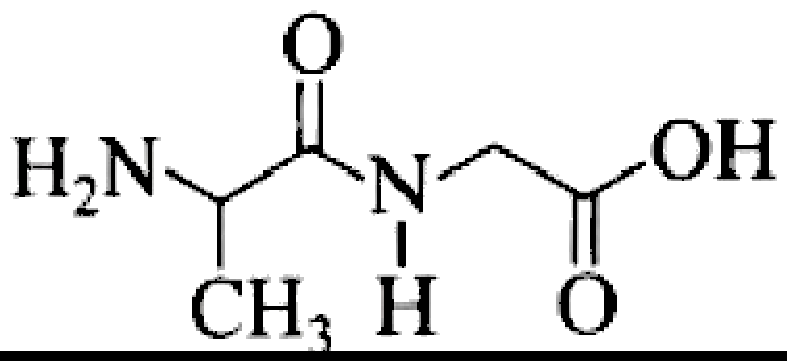
\includegraphics[width=4.5cm]{images_crop_de07/cau14_dipeptide.png}\par}
Khi thuỷ phân hoàn toàn X trong môi trường NaOH thu được sản phẩm hữu cơ có công thức là
\choice
{\ce{H2NCH(CH3)COOH} và \ce{H2NCH2COOH}}
{\ce{H2NCH(CH3)COONa} và \ce{H2NCH2COONa}}
{\ce{H2NCH(CH3)COONa} và \ce{H2NCH2COOH}}
{\ce{H2NCH(CH3)COOH} và \ce{H2NCH2COONa}}
\loigiai{}
\end{ex}

\begin{ex}
(SBT -- CĐ). Leucine có công thức cấu tạo \ce{HOOCCH(NH2)CH2CH(CH3)2}, là amino acid có khả năng điều hòa sự tổng hợp protein của cơ. Tên theo danh pháp thay thế của leucine là
\choice
{2-aminoisohexanoic acid}
{2-amino-4-methylpentanoic acid}
{4-amino-2-methylpentanoic acid}
{2-amino-isohexanoic acid}
\loigiai{}
\end{ex}

\begin{ex}
(SBT -- CTST). Dung dịch của chất nào sau đây có môi trường base?
{\centering
	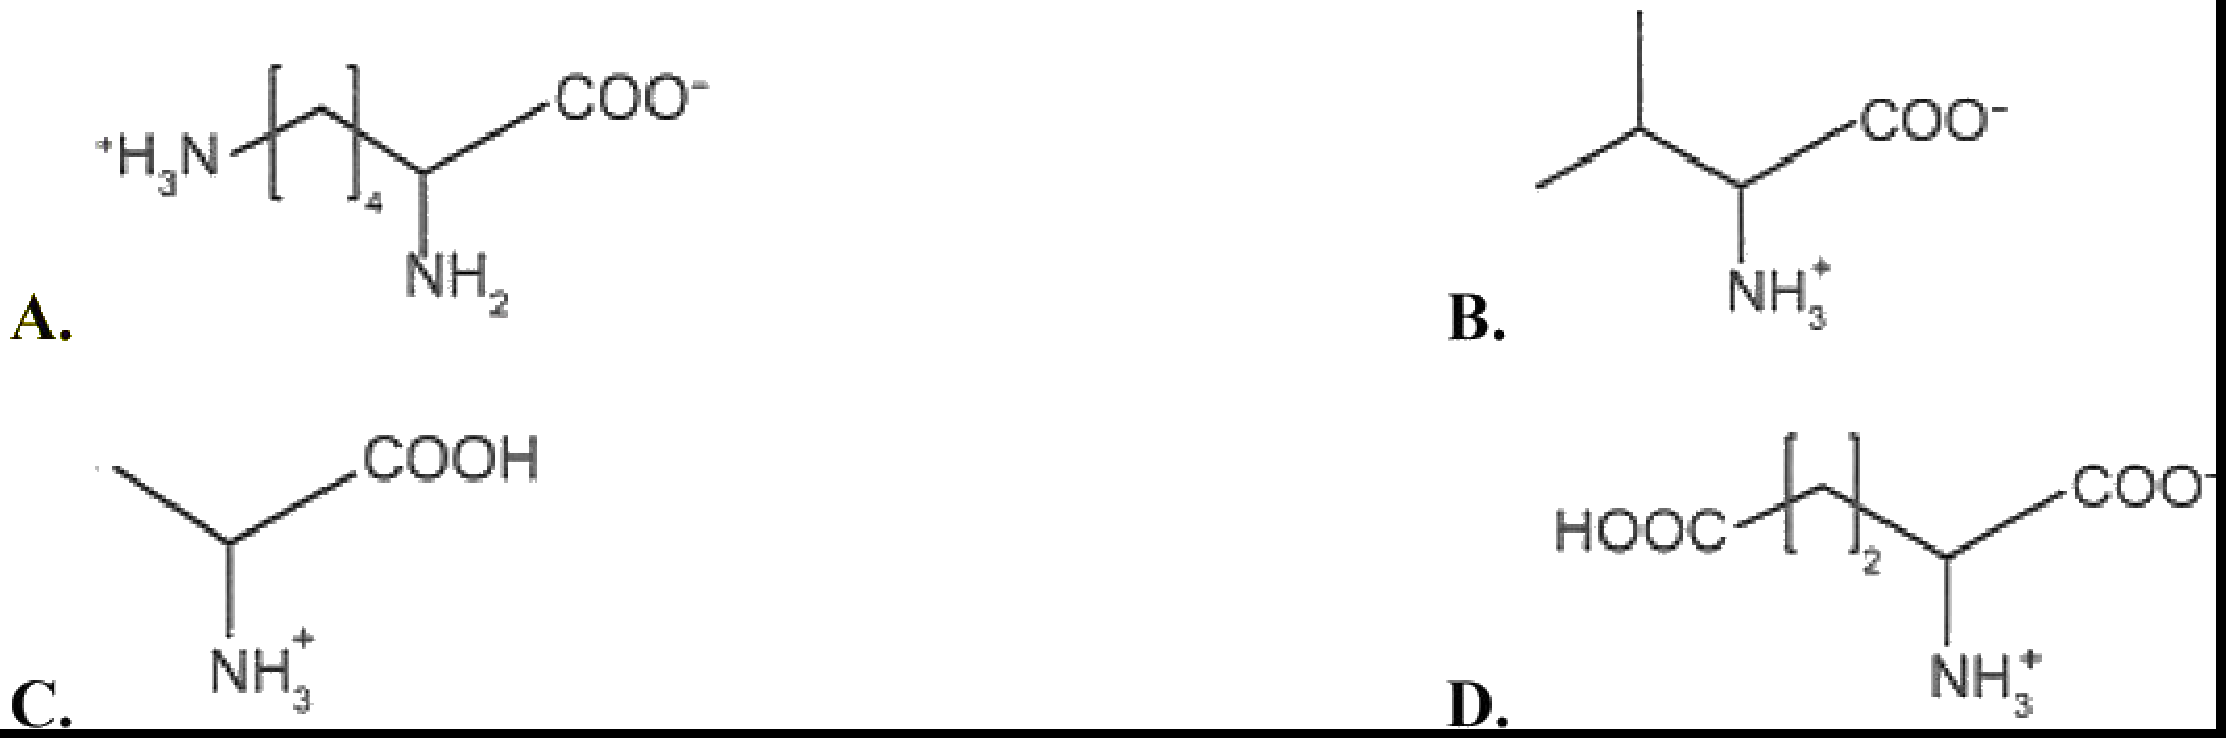
\includegraphics[width=10.5cm]{images_crop_de07/cau16_options.png}\par}
\loigiai{}
\end{ex}

\begin{ex}
(SBT -- CTST). Nguyên nhân chủ yếu dẫn đến tính tan của amino acid trong nước là do
\choice
{phân tử phân cực mạnh nên dễ tan trong nước}
{cấu tạo lưỡng cực của phân tử, có tính kị nước nên ít tan trong nước}
{năng lượng liên kết của phân tử lớn, khó phá vỡ nên ít tan trong nước}
{hình thành liên kết hydrogen với nước nên dễ tan trong nước}
\loigiai{}
\end{ex}

\begin{ex}
Cho các phát biểu sau:\\
(a) Phenylamine có lực base yếu hơn ammonia.\\
(b) Phenylamine tan ít trong nước nhưng tan tốt trong dung dịch HCl.\\
(c) Khi nấu canh cua, hiện tượng riêu cua nổi lên trên là do sự đông tụ protein.\\
(d) Trong tơ tằm có các gốc $\alpha$-amino acid.\\
(e) Dùng giấm ăn hoặc chanh khử được mùi tanh trong cá do amine gây ra.\\
Số phát biểu đúng là
\choice
{5}
{2}
{3}
{4}
\loigiai{}
\end{ex}

\Closesolutionfile{ans}

\newpage

\vspace{0.15cm}
\noindent
\textbf{PHẦN II (4,0 điểm -- 4 câu): Câu trắc nghiệm đúng sai.}\\
\textit{Thí sinh trả lời từ câu 1 đến câu 4. Trong mỗi ý a), b), c), d) ở mỗi câu, thí sinh chọn đúng hoặc sai.}

\setcounter{ex}{0}

\begin{ex}
(SBT -- KNTT). Các phát biểu về điều chế và ứng dụng của amine:
\choiceTF
{Một số amine có thể được điều chế bằng cách alkyl hoá ammonia}
{Một số amine có thể được điều chế bằng cách khử hợp chất nitro}
{Amine được sử dụng để tổng hợp một số loại dược phẩm}
{Amine được sử dụng để tổng hợp một số loại polymer}
\loigiai{}
\end{ex}

\begin{ex}
(SBT -- CTST). Cho một số hợp chất chứa nguyên tố nitrogen như hình bên dưới:\\
Về tính chất hoá học của các chất, hãy cho biết các phát biểu sau đúng hay sai:
{\centering
	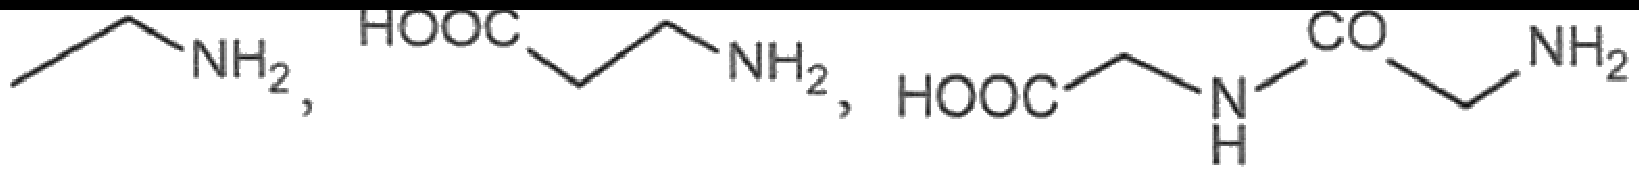
\includegraphics[width=9.5cm]{images_crop_de07/p2_cau2_compounds.png}\par}
\choiceTF
{Đều có phản ứng với dung dịch HCl, sinh ra muối}
{Có 1 chất tham gia phản ứng thuỷ phân}
{Có thể trùng ngưng tạo thành peptide}
{Chỉ tạo phức với \ce{Cu(OH)2} tạo thành dung dịch có màu xanh}
\loigiai{}
\end{ex}

\begin{ex}
Collagen được coi là một loại protein quan trọng đối với làn da, trong đó peptide lại có vai trò lớn thúc đẩy sản xuất collagen. Điều này giải thích cho việc peptide có khả năng chống lại sự lão hóa, giúp làm mờ các vết nhăn làm làn da luôn căng mịn.
\choiceTF
{Trong một phân tử tetrapeptide mạch hở có 4 liên kết peptide}
{Peptide là loại hợp chất chứa gốc $\alpha$-amino acid}
{Trong môi trường base, dipeptide mạch hở tác dụng được với \ce{Cu(OH)2} cho hợp chất màu tím}
{Các hợp chất peptide kém bền trong môi trường base nhưng bền trong môi trường acid}
\loigiai{}
\end{ex}

\begin{ex}
Thành phần tạo nên vị ngọt đặc trưng của nước mắm (được sản xuất từ cá) và nước tương (được sản xuất từ đậu nành) là các amino acid tạo thành từ sự thuỷ phân hoàn toàn của protein có trong cá hoặc đậu nành.
\choiceTF
{Độ đạm tương ứng với hàm lượng oxygen có trong nước mắm, nước tương}
{Độ đạm có tỉ lệ thuận với hàm lượng amino acid có trong nước mắm, nước tương}
{Vì hàm lượng nitrogen quyết định đến độ đạm trong khi nitrogen có trong thành phần của amino acid nên độ đạm có tỉ lệ nghịch với hàm lượng amino acid}
{Độ đạm trong nước mắm là quá trình thủy phân cá, các chất protein được thủy phân tạo thành các amino acid nước mắm sẽ có mùi thơm đặc trưng riêng}
\loigiai{}
\end{ex}

\newpage

\vspace{0.15cm}
\noindent
\textbf{PHẦN III (1,5 điểm -- 6 câu): Câu trắc nghiệm yêu cầu trả lời ngắn.}\\
\textit{Thí sinh trả lời từ câu 1 đến câu 6. Mỗi câu hỏi thí sinh điền câu trả lời vào ô tương ứng.}

\setcounter{ex}{0}

\begin{ex}
Cho dãy các chất: \ce{H2NCH2COOH}, \ce{HCOONH4}, \ce{(CH3NH3)2CO3}, \ce{C6H5NH2}, \ce{C2H5NH2}, \ce{CH3COOH}, \ce{H2NCH2CONHCH(CH3)COOH}. Số lượng chất trong dãy phản ứng được với cả 2 dung dịch NaOH và dung dịch HCl là
\loigiai{}
\end{ex}
\noindent\textit{Đáp số:} \dotfill\vspace{0.25cm}

\begin{ex}
Cho các chất sau: \ce{CH3COONH4}, \ce{CH3COONH3CH3}, \ce{C2H5NH2}, \ce{H2NCH2COOC2H5}. Số chất trong dãy vừa tác dụng được với NaOH và vừa tác dụng được với HCl trong dung dịch là:
\loigiai{}
\end{ex}
\noindent\textit{Đáp số:} \dotfill\vspace{0.25cm}

\begin{ex}
Nếu thuỷ phân không hoàn toàn pentapeptide Gly-Ala-Gly-Ala-Gly thì thu được tối đa bao nhiêu dipeptide khác nhau?
\loigiai{}
\end{ex}
\noindent\textit{Đáp số:} \dotfill\vspace{0.25cm}

\begin{ex}
Tiến hành thí nghiệm phản ứng màu biuret của lòng trắng trứng (protein) theo các bước sau đây:\\
\textit{Bước 1:} Cho vào ống nghiệm 1 giọt dung dịch \ce{CuSO4} 2\% + 1 mL dung dịch NaOH 30\%.\\
\textit{Bước 2:} Lắc nhẹ, gạn lớp dung dịch để giữ kết tủa.\\
\textit{Bước 3:} Thêm 4 mL dung dịch lòng trắng trứng vào ống nghiệm, lắc đều.\\
Cho các nhận định sau:\\
(1) Cần lấy dư dung dịch NaOH để đảm bảo môi trường cho phản ứng tạo phức.\\
(2) Có thể thay thế dung dịch lòng trắng trứng bằng dung dịch Gly-Ala.\\
(3) Sau bước 3, kết tủa bị hoà tan và dung dịch có màu tím đặc trưng.\\
(4) Sau bước 1, trong ống nghiệm xuất hiện kết tủa màu xanh lam.\\
Có bao nhiêu nhận định đúng trong các nhận định trên?
\loigiai{}
\end{ex}
\noindent\textit{Đáp số:} \dotfill\vspace{0.25cm}

\begin{ex}
Xác định phân tử khối gần đúng của một hemoglobin (huyết cầu tố) chứa 0,4\% Fe về khối lượng (mỗi phân tử hemoglobin chỉ chứa 1 nguyên tử iron).
\loigiai{}
\end{ex}
\noindent\textit{Đáp số:} \dotfill\vspace{0.25cm}

\begin{ex}
Một khẩu phần thịt gà nướng 100g chứa khoảng 25g protein. Một người trong ngày đã ăn 150g thịt gà, 200g cá hồi (chứa 22g protein/100g) và 50g phô mai (chứa 7g protein/100g). Hãy tính tổng lượng protein (theo đơn vị gram) người đó đã hấp thụ từ các thực phẩm này.
\loigiai{}
\end{ex}
\noindent\textit{Đáp số:} \dotfill\vspace{0.25cm}

\vspace{0.1cm}
\begin{center}
	\textbf{---------- HẾT ----------}
\end{center}

\end{document}
